% 
% 	ondas_planas_raio.tex (LATEX)
% 
% 	Objetivo: Estudo sobre básico da teoria do raio.
%
%	Versão 1.0
% 
% 	Programador: Rodolfo A. C. Neves (Dirack) 23/01/2020
% 
%	Licensa: Software de uso livre e gratuito.

\documentclass[a4paper, 12pt]{article}

% Pacotes fundamentais
  \usepackage{multirow}
  \usepackage[top=2cm, bottom=2cm, left=2.5cm, right=2.5cm]{geometry}
  \usepackage[utf8]{inputenc}
  \usepackage{amsmath, amsfonts, amssymb}
  \usepackage{float}
  \usepackage{graphicx}
  \usepackage[portuguese]{babel}

\begin{document}

\section{A teoria do raio em um modelo de ondas planas: Vagarosidade horizontal}

\begin{figure}[H]
\caption{Exemplo esquemático de uma onda plana atingindo a superfície de aquisição formando um ângulo $\theta$
com a normal à superfície. Apresentamos dois instantâneos da propagação da onda plana, $t$ e $t + \Delta t$.
A velocidade do meio é constante e igual a $v$.}
\begin{center}
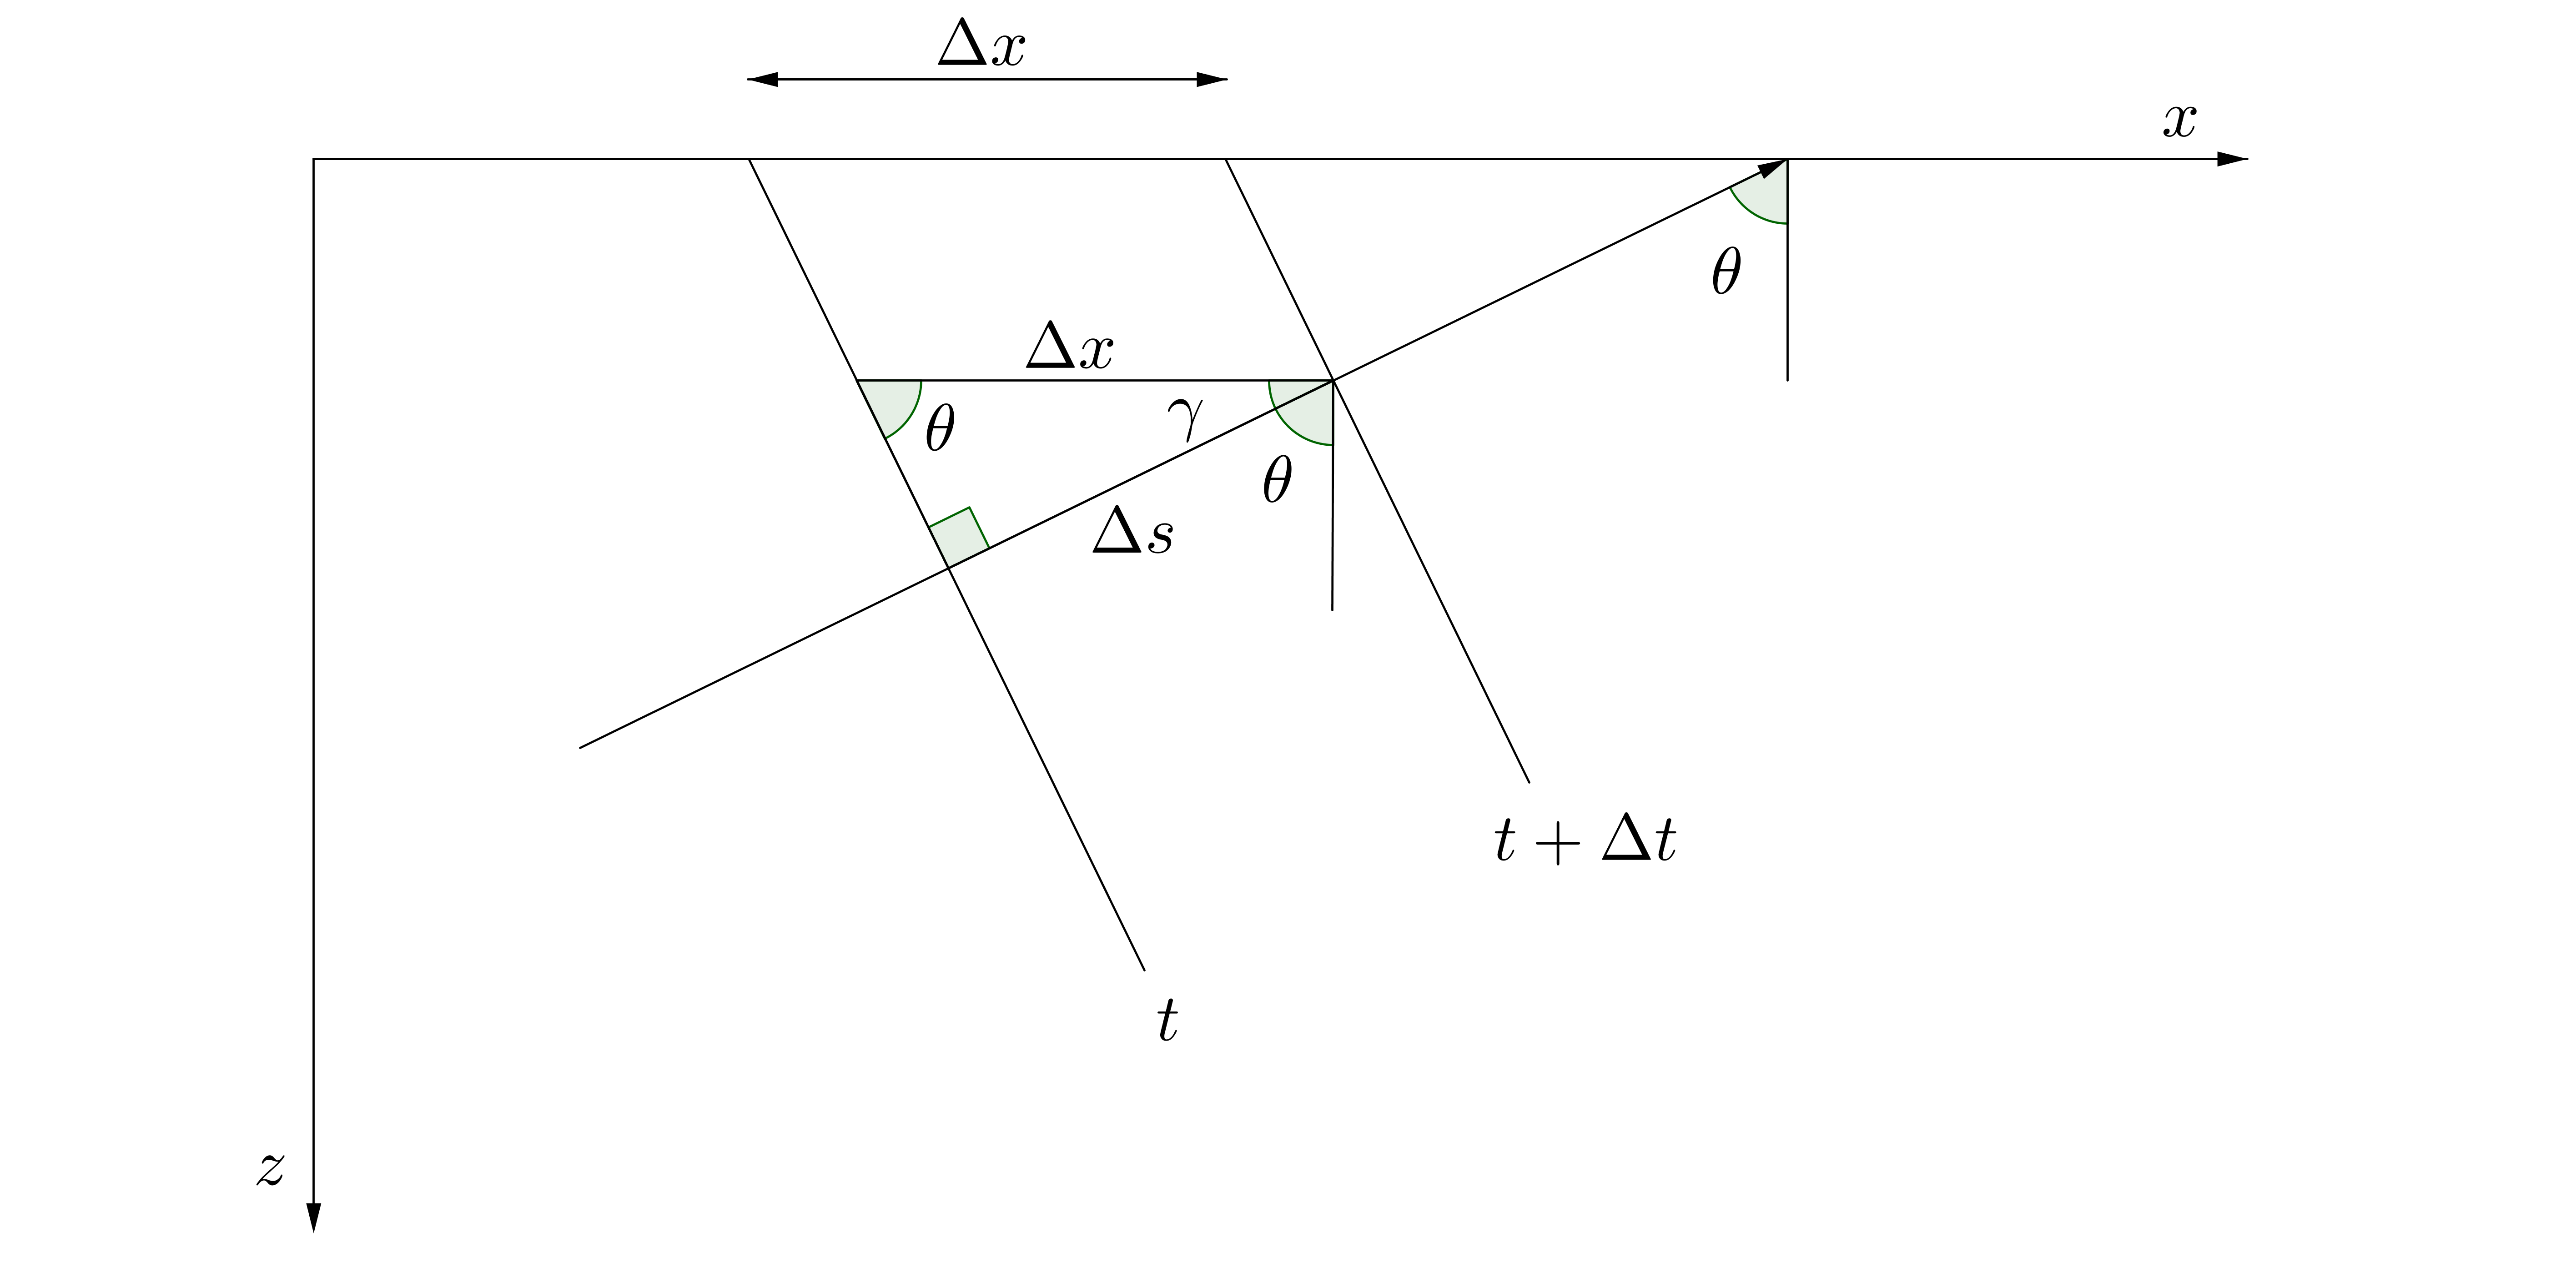
\includegraphics[scale=0.7]{images/raio_ondas_planas.png}
\vspace{-0.3cm}
\end{center}
\begin{center}
 Fonte: Do Autor.
\end{center}
\label{fig:1.1}
\end{figure}

O espaço $\Delta s$ percorrido pela onda plana do tempo $t$ a $t + \Delta t$:

\begin{equation}
\label{eq:1.1}
\Delta s = \Delta x \cos \gamma = \Delta x \sin \theta
\end{equation}

Pois:

\begin{equation}
\label{eq:1.2}
\gamma = \frac{\pi}{2} - \theta
\end{equation}

\begin{equation}
\label{eq:1.3}
\cos \gamma = \cos \left( \frac{\pi}{2} - \theta \right)
\end{equation}

\begin{equation}
\label{eq:1.4}
\cos \gamma = \cos \frac{\pi}{2} \cos \theta + \sin \theta \sin \frac{\pi}{2}
\end{equation}

Por definição $\cos \frac{\pi}{2} = 1$ e $\sin \frac{\pi}{2} = 0$:

\begin{equation}
\label{eq:1.5}
\cos \gamma = \sin \theta
\end{equation}

A velocidade da onda plana no meio:

\begin{equation}
 \label{eq:1.6}
 v = \frac{\Delta s}{\Delta t} = \frac{\Delta x \sin \theta}{\Delta t}
\end{equation}

\begin{equation}
 \label{eq:1.7}
 v \Delta t = \Delta x \sin \theta
\end{equation}

\begin{equation}
 \label{eq:1.8}
 \frac{\Delta t}{\Delta x} = \frac{\sin \theta}{v} = u \sin \theta \equiv p
\end{equation}

A vagarosidade é definida como $u=1/v$, $p$ é a chamada vagarosidade horizontal.

\section{Sistema centrado no raio: Vagarosidade vertical}

\begin{equation}
 \label{eq:1.9}
 \eta = u \cos \theta = (u^2 - p^2)^{1/2}
\end{equation}

Pois:

\begin{equation}
 \label{eq:1.10}
 u^2 = p^2 + \eta^2
\end{equation}

Notar que no \textit{turning point}, $p=u$ e $\eta=0$:


\begin{equation}
 \label{eq:1.11}
 \frac{dx}{ds} = \sin \theta = \frac{p}{u}
\end{equation}

\begin{equation}
 \label{eq:1.12}
 \frac{dz}{ds} = \cos \theta = (1 - \sin^2\theta)^{1/2} = (1 - p^2/u^2)^{1/2} = u^{-1}(u^2 - p^2)^{1/2}
\end{equation}

Da regra da cadeia:

\begin{equation}
 \label{eq:1.13}
 \frac{dx}{dz} = \frac{dx}{ds} \frac{ds}{dz} = \frac{p}{u} \frac{u}{(u^2-p^2)^{1/2}} = \frac{p}{(u^2-p^2)^{1/2}}
\end{equation}




\end{document}